We present a double integrator example, with state $(x_1, x_2)$, control $u \in [u_{min}, u_{max}]$ and disturbance $d \in [d_{min}, d_{max}]$ with dynamics,
\begin{equation}
\begin{split}
\dot{x_1} & = x_2 \\
\dot{x_2} & = u \cdot(u_{max}-u_{min}) + u_{min} + d \cdot (d_{max}-d_{min}) + d_{min}
\end{split}
\end{equation}
In our experiments, we discretize the state space, to a $161 \times 161$ grid; control space and disturbance space. 

We first show, in Fig~\ref{fig:convergence} that $Z$ over approximates~(bold line) and under approximates~(dotted lines) the true reachable set~(shown in black) for two values of $\lambda = 0.1, 0.2$. The target set $\mathcal{T}$ is shown in red. 
\begin{figure}
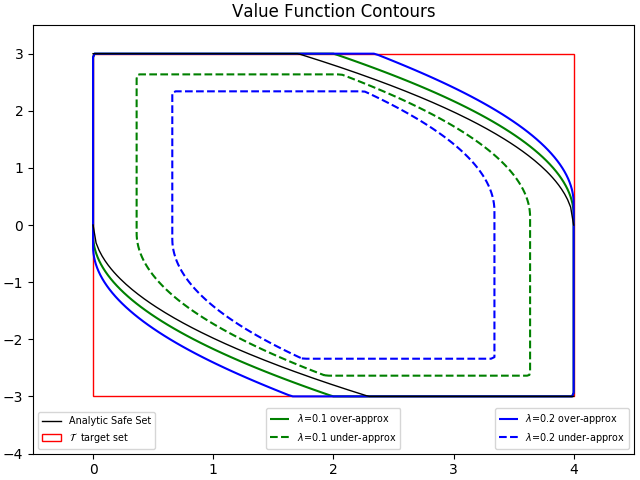
\includegraphics[scale=0.5]{convergence_difflambda.png}
\caption{The analytic reachable set $V$ and target set $\mathcal{T}$ are shown in black and red. The over and under approximated $Z_{\lambda}$ are shown in bold green and dotted green for $\lambda=0.1$; and bold blue and dotted blue line for $\lambda  = 0.2$. This suggests smaller the value of $\lambda$, the better $Z_{\lambda}$ approximates $V$.}
\label{fig:convergence}
\end{figure}

We next compare value iteration and policy iteration with increasing number of discrete actions in Table~\ref{tab:v_vs_p}. In the table we see that as the number of actions increase, there is sharp increase in how long value iteration takes to converge ($T^{v}_{conv}$)  while the increase is much smaller for policy iteration ($T^{p}_{conv}$). However, the total time ($T_{total}$) taken for policy iteration is much larger since there is a significant overhead in building the matrices for value functions. 
\begin{table}
\centering
\caption{Value Iteration vs Policy Iteration}
\label{tab:v_vs_p}
\begin{tabular}{|c| c| c| c| c| c|}
\hline
\# of & \multicolumn{2}{|c|}{Value Iteration} & \multicolumn{3}{|c|}{Policy Iteration} \\ \cline{2-6}
Actions & Iters & $T^{v}_{conv}$ & Iters & $T_{total}$ & $T^{p}_{conv}$ \\ \hline
2 & 204 & 1.255 & 4 & 68.793 & 0.105 \\ \hline
50 & 204 & 7.562 & 4 & 69.717 & 0.365 \\ \hline
250 & 204 & 32.841 & 14 & 251.39 & 3.504 \\ \hline
500 & 204 & 63.815 & 14 & 253.855 & 6.741 \\
\hline
\end{tabular}
\end{table}

Finally, we ran value iteration from different initializations, the signed distance function $Z_0 = l(\cdot)$ and an all zeros $Z_0= 0$. The converged values functions had a norm of $0.000299$ between them, suggesting that MDR converges independent of the initialization. However, running MR with $V_0 = 0$, does not converge to the true value function.